\documentclass{standalone}
\usepackage{tikz}
\usetikzlibrary{patterns, positioning}

\begin{document}
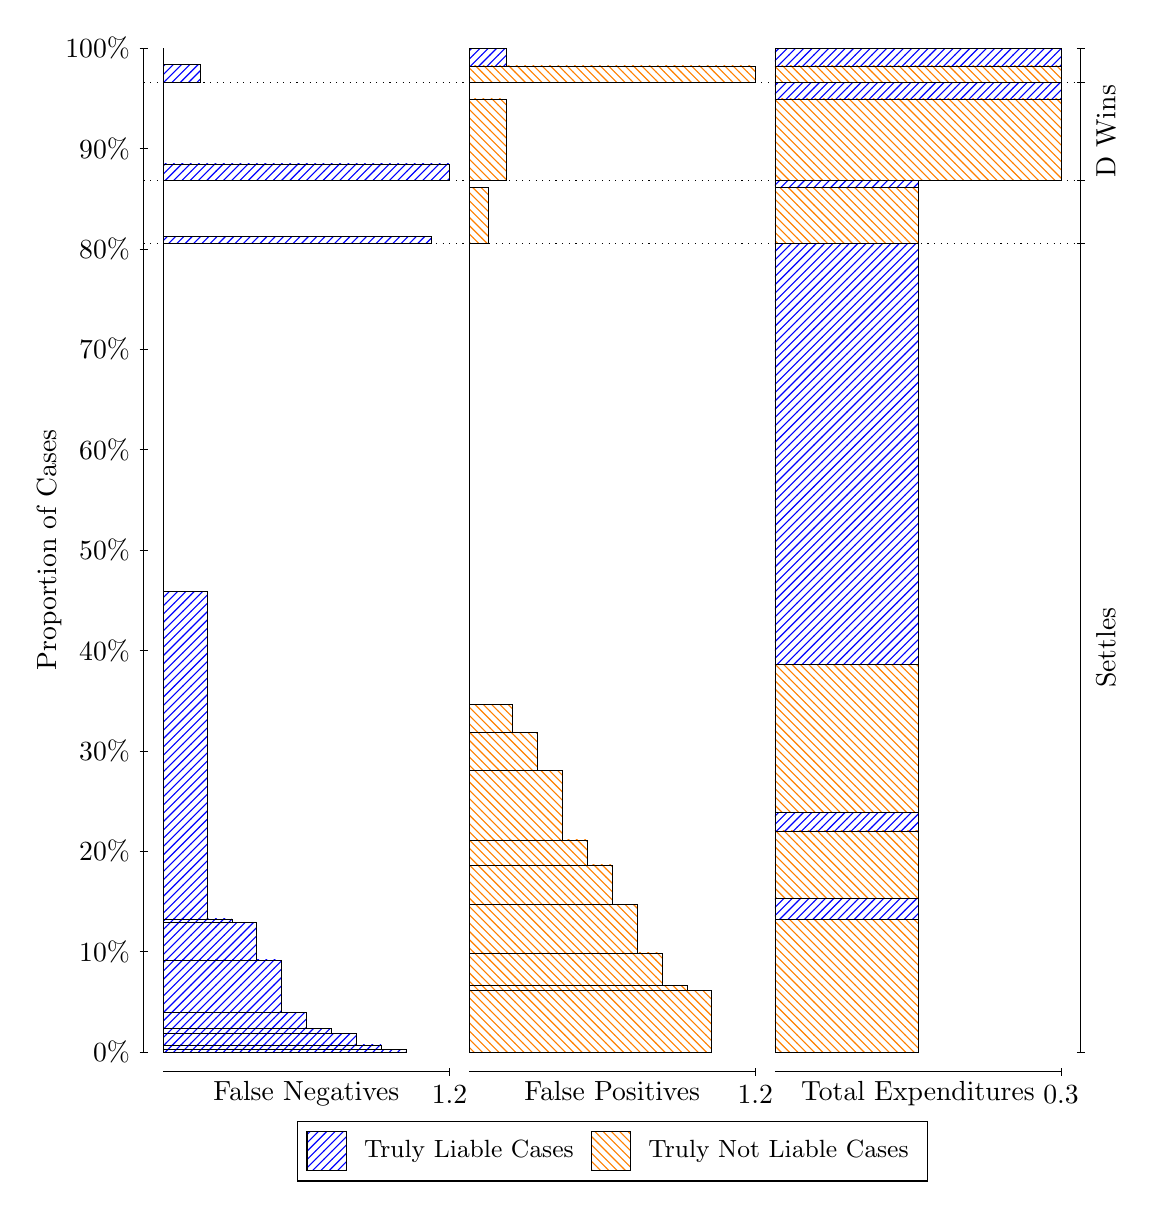
\begin{tikzpicture}
\draw[black, very thin] (1.5,1.75) -- (1.5,14.5);
\node[rotate=90, anchor=center] at (0.3, 8.125) {Proportion of Cases};
\draw[black, very thin] (1.45,1.75) -- (1.55,1.75);
\node[anchor=east] at (1.45, 1.75) {0\%};
\draw[black, very thin] (1.45,3.025) -- (1.55,3.025);
\node[anchor=east] at (1.45, 3.025) {10\%};
\draw[black, very thin] (1.45,4.3) -- (1.55,4.3);
\node[anchor=east] at (1.45, 4.3) {20\%};
\draw[black, very thin] (1.45,5.575) -- (1.55,5.575);
\node[anchor=east] at (1.45, 5.575) {30\%};
\draw[black, very thin] (1.45,6.85) -- (1.55,6.85);
\node[anchor=east] at (1.45, 6.85) {40\%};
\draw[black, very thin] (1.45,8.125) -- (1.55,8.125);
\node[anchor=east] at (1.45, 8.125) {50\%};
\draw[black, very thin] (1.45,9.4) -- (1.55,9.4);
\node[anchor=east] at (1.45, 9.4) {60\%};
\draw[black, very thin] (1.45,10.675) -- (1.55,10.675);
\node[anchor=east] at (1.45, 10.675) {70\%};
\draw[black, very thin] (1.45,11.95) -- (1.55,11.95);
\node[anchor=east] at (1.45, 11.95) {80\%};
\draw[black, very thin] (1.45,13.225) -- (1.55,13.225);
\node[anchor=east] at (1.45, 13.225) {90\%};
\draw[black, very thin] (1.45,14.5) -- (1.55,14.5);
\node[anchor=east] at (1.45, 14.5) {100\%};

\draw[black, very thin] (13.4,1.75) -- (13.4,14.5);
\draw[black, very thin] (13.35,1.75) -- (13.45,1.75);
\node[anchor=west] at (13.35, 1.75) {};
\draw[black, very thin] (13.35,12.016) -- (13.45,12.016);
\node[anchor=west] at (13.35, 12.016) {};
\draw[black, very thin] (13.35,12.817) -- (13.45,12.817);
\node[anchor=west] at (13.35, 12.817) {};
\draw[black, very thin] (13.35,14.066) -- (13.45,14.066);
\node[anchor=west] at (13.35, 14.066) {};
\draw[black, very thin] (13.35,14.5) -- (13.45,14.5);
\node[anchor=west] at (13.35, 14.5) {};

\draw[black, very thin, pattern color=blue, pattern=north east lines] (1.75,1.75) rectangle (4.8304,1.7865);
\draw[black, very thin, pattern color=blue, pattern=north east lines] (1.75,1.7865) rectangle (4.5145,1.8412);
\draw[black, very thin, pattern color=blue, pattern=north east lines] (1.75,1.8412) rectangle (4.1986,1.9872);
\draw[black, very thin, pattern color=blue, pattern=north east lines] (1.75,1.9872) rectangle (3.8826,2.054);
\draw[black, very thin, pattern color=blue, pattern=north east lines] (1.75,2.054) rectangle (3.5667,2.2513);
\draw[black, very thin, pattern color=blue, pattern=north east lines] (1.75,2.2513) rectangle (3.2507,2.9182);
\draw[black, very thin, pattern color=blue, pattern=north east lines] (1.75,2.9182) rectangle (2.9348,3.393);
\draw[black, very thin, pattern color=blue, pattern=north east lines] (1.75,3.393) rectangle (2.6188,3.4395);
\draw[black, very thin, pattern color=blue, pattern=north east lines] (1.75,3.4395) rectangle (2.3029,7.5996);
\draw[black, very thin, pattern color=orange, pattern=north west lines] (1.75,7.5996) rectangle (1.75,12.016);
\draw[black, very thin, pattern color=blue, pattern=north east lines] (1.75,12.016) rectangle (5.1464,12.103);
\draw[black, very thin, pattern color=orange, pattern=north west lines] (1.75,12.103) rectangle (1.75,12.817);
\draw[black, very thin, pattern color=blue, pattern=north east lines] (1.75,12.817) rectangle (5.3833,13.029);
\draw[black, very thin, pattern color=orange, pattern=north west lines] (1.75,13.029) rectangle (1.75,14.066);
\draw[black, very thin, pattern color=blue, pattern=north east lines] (1.75,14.066) rectangle (2.2239,14.292);
\draw[black, very thin, pattern color=orange, pattern=north west lines] (1.75,14.292) rectangle (1.75,14.5);
\draw[black, very thin, pattern color=orange, pattern=north west lines] (5.6333,1.75) rectangle (8.7138,2.5312);
\draw[black, very thin, pattern color=orange, pattern=north west lines] (5.6333,2.5312) rectangle (8.3978,2.5937);
\draw[black, very thin, pattern color=orange, pattern=north west lines] (5.6333,2.5937) rectangle (8.0819,3.0084);
\draw[black, very thin, pattern color=orange, pattern=north west lines] (5.6333,3.0084) rectangle (7.7659,3.6263);
\draw[black, very thin, pattern color=orange, pattern=north west lines] (5.6333,3.6263) rectangle (7.45,4.1257);
\draw[black, very thin, pattern color=orange, pattern=north west lines] (5.6333,4.1257) rectangle (7.1341,4.4431);
\draw[black, very thin, pattern color=orange, pattern=north west lines] (5.6333,4.4431) rectangle (6.8181,5.3303);
\draw[black, very thin, pattern color=orange, pattern=north west lines] (5.6333,5.3303) rectangle (6.5022,5.8049);
\draw[black, very thin, pattern color=orange, pattern=north west lines] (5.6333,5.8049) rectangle (6.1862,6.1662);
\draw[black, very thin, pattern color=blue, pattern=north east lines] (5.6333,6.1662) rectangle (5.6333,12.016);
\draw[black, very thin, pattern color=orange, pattern=north west lines] (5.6333,12.016) rectangle (5.8703,12.73);
\draw[black, very thin, pattern color=blue, pattern=north east lines] (5.6333,12.73) rectangle (5.6333,12.817);
\draw[black, very thin, pattern color=orange, pattern=north west lines] (5.6333,12.817) rectangle (6.1072,13.854);
\draw[black, very thin, pattern color=blue, pattern=north east lines] (5.6333,13.854) rectangle (5.6333,14.066);
\draw[black, very thin, pattern color=orange, pattern=north west lines] (5.6333,14.066) rectangle (9.2667,14.274);
\draw[black, very thin, pattern color=blue, pattern=north east lines] (5.6333,14.274) rectangle (6.1072,14.5);
\draw[black, very thin, pattern color=orange, pattern=north west lines] (9.5167,1.75) rectangle (11.333,3.4292);
\draw[black, very thin, pattern color=blue, pattern=north east lines] (9.5167,3.4292) rectangle (11.333,3.6968);
\draw[black, very thin, pattern color=orange, pattern=north west lines] (9.5167,3.6968) rectangle (11.333,4.5575);
\draw[black, very thin, pattern color=blue, pattern=north east lines] (9.5167,4.5575) rectangle (11.333,4.7913);
\draw[black, very thin, pattern color=orange, pattern=north west lines] (9.5167,4.7913) rectangle (11.333,6.6676);
\draw[black, very thin, pattern color=blue, pattern=north east lines] (9.5167,6.6676) rectangle (11.333,12.016);
\draw[black, very thin, pattern color=orange, pattern=north west lines] (9.5167,12.016) rectangle (11.333,12.73);
\draw[black, very thin, pattern color=blue, pattern=north east lines] (9.5167,12.73) rectangle (11.333,12.817);
\draw[black, very thin, pattern color=orange, pattern=north west lines] (9.5167,12.817) rectangle (13.15,13.854);
\draw[black, very thin, pattern color=blue, pattern=north east lines] (9.5167,13.854) rectangle (13.15,14.066);
\draw[black, very thin, pattern color=orange, pattern=north west lines] (9.5167,14.066) rectangle (13.15,14.274);
\draw[black, very thin, pattern color=blue, pattern=north east lines] (9.5167,14.274) rectangle (13.15,14.5);
\draw[black, dotted] (1.5,12.016) -- (13.4,12.016);
\draw[black, dotted] (1.5,12.817) -- (13.4,12.817);
\draw[black, dotted] (1.5,14.066) -- (13.4,14.066);
\draw[black, very thin] (1.75,1.5) -- (5.3833,1.5);
\node[anchor=north] at (3.5667, 1.5) {False Negatives};
\draw[black, very thin] (5.3833,1.45) -- (5.3833,1.55);
\node[anchor=north] at (5.3833, 1.45) {1.2};

\draw[black, very thin] (5.6333,1.5) -- (9.2667,1.5);
\node[anchor=north] at (7.45, 1.5) {False Positives};
\draw[black, very thin] (9.2667,1.45) -- (9.2667,1.55);
\node[anchor=north] at (9.2667, 1.45) {1.2};

\draw[black, very thin] (9.5167,1.5) -- (13.15,1.5);
\node[anchor=north] at (11.333, 1.5) {Total Expenditures};
\draw[black, very thin] (13.15,1.45) -- (13.15,1.55);
\node[anchor=north] at (13.15, 1.45) {0.3};

\node[black, centered, rotate=90] at (13.72, 6.8829) {Settles};

\node[black, centered, rotate=90] at (13.72, 13.441) {D Wins};


\draw (7.449999999999999,1.5) node[draw=none] (baseCoordinate) {};
\begin{scope}[align=center]
        \matrix[scale=0.5, draw=black, below=0.5cm of baseCoordinate, nodes={draw}, column sep=0.1cm]{
            \node[rectangle, draw, minimum width=0.5cm, minimum height=0.5cm, pattern=north east lines, pattern color=blue] {}; &
            \node[draw=none, font=\small] (B) {Truly Liable Cases}; &
            \node[rectangle, draw, minimum width=0.5cm, minimum height=0.5cm, pattern=north west lines, pattern color=orange] {}; &
            \node[draw=none, font=\small] (B) {Truly Not Liable Cases}; \\
            };
\end{scope}

\end{tikzpicture}
\end{document}